\documentclass[conference]{IEEEtran}
\IEEEoverridecommandlockouts
% The preceding line is only needed to identify funding in the first footnote. If that is unneeded, please comment it out.
\usepackage{cite}
\usepackage{amsmath,amssymb,amsfonts}
\usepackage{algorithmic}
\usepackage{graphicx}
\usepackage{textcomp}
\usepackage{xcolor}
\usepackage{hyperref}
\usepackage{enumerate}  %枚举的符号
\usepackage{geometry}   %页面形式
\usepackage{fancyhdr}   % 设置页眉
\usepackage{xcolor} %颜色
\usepackage{listings}   %插入代码
\usepackage{amsmath}
\usepackage{mathtools}
\usepackage{amsthm}
\usepackage{amssymb}
\usepackage{amsfonts}
\usepackage{longtable}  %长表格
\usepackage[all,cmtip]{xy}  %交换图
\usepackage{pgf,tikz}   %自动机画图
\usetikzlibrary{shapes,arrows,automata}
\usepackage{graphicx}

% \usepackage{algorithm}  %算法
% \usepackage{algpseudocode}
\usepackage{graphics}
\usepackage{epsfig}
%算法中用\require, \ensure写input,output
% \renewcommand{\algorithmicrequire}{\textbf{Input:}} % Use Input in the format of Algorithm
% \renewcommand{\algorithmicensure}{\textbf{Output:}} % Use Output in the format of Algorithm
% \newcommand{\algorithmiclastcon}{\textbf{Initialize:}}
% \newcommand{\Initialize}{\item[\algorithmiclastcon]}

\usepackage{framed} %给文字加框

\usepackage{bm} %给数学公式中的符号加粗
\usepackage{bbm}

\usepackage{yhmath} %把\Widehat命令设为自动调整大小的hat符号
\DeclareSymbolFont{largesymbol}{OMX}{yhex}{m}{n}
\DeclareMathAccent{\Widehat}{\mathord}{largesymbol}{"62}

\renewcommand\tablename{Table}  %设置图表的名字
\renewcommand\figurename{Figure}
% \CTEXoptions[today=old] %设置日期为英文
\renewcommand\refname{Reference}    % 设置参考文献为英文

\setlength{\parindent}{0pt} %设置不缩进
\linespread{1}  % 改变行距

% \usepackage[T1]{fontenc} %  textsc
\usepackage{xspace}
\usepackage{enumitem}

\usepackage{todonotes}

\usepackage{multirow}
\usepackage{booktabs}





\newtheorem{problem}{Problem}
\newtheorem{lemma}{Lemma}
\newtheorem{theorem}[lemma]{Theorem}
\newtheorem{corollary}[lemma]{Corollary}
\newtheorem{proposition}[lemma]{Proposition}
\newtheorem{definition}[lemma]{Definition}
\newtheorem{property}{Property}
\newtheorem{assumption}{Assumption}
\newtheorem{conjecture}{Conjecture}
\newtheorem*{exercise}{Exercise}
\newtheorem*{remark}{Remark}
\newtheorem*{observation}{Observation}
\newtheorem*{example}{Example}
\newtheorem*{solution}{Solution}
\newtheorem*{notation}{Notation}
\newtheorem*{question}{Question}
% \newtheorem*{conjecture}{Conjecture}


% notations
\newcommand{\wt}[1]{\widetilde{#1}}
\newcommand{\h}[1]{\Widehat{#1}}
\renewcommand{\o}[1]{\overline{#1}}
\renewcommand{\u}[1]{\underline{#1}}
\newcommand{\s}[1]{\sqrt{#1}}
\renewcommand{\d}{\textnormal{d}}
\newcommand{\tto}{\Rightarrow}


% formatting
\newcommand\blankline{~\\}



\newcommand{\cA}{\mathcal{A}}
\newcommand{\cB}{\mathcal{B}}
\newcommand{\cC}{\mathcal{C}}
\newcommand{\cD}{\mathcal{D}}
\newcommand{\cE}{\mathcal{E}}
\newcommand{\cF}{\mathcal{F}}
\newcommand{\cG}{\mathcal{G}}
\newcommand{\cH}{\mathcal{H}}
\newcommand{\cI}{\mathcal{I}}
\newcommand{\cJ}{\mathcal{J}}
\newcommand{\cK}{\mathcal{K}}
\newcommand{\cL}{\mathcal{L}}
\newcommand{\cM}{\mathcal{M}}
\newcommand{\cN}{\mathcal{N}}
\newcommand{\cO}{\mathcal{O}}
\newcommand{\cP}{\mathcal{P}}
\newcommand{\cQ}{\mathcal{Q}}
\newcommand{\cR}{\mathcal{R}}
\newcommand{\cS}{\mathcal{S}}
\newcommand{\cT}{\mathcal{T}}
\newcommand{\cU}{\mathcal{U}}
\newcommand{\cV}{\mathcal{V}}
\newcommand{\cW}{\mathcal{W}}
\newcommand{\cX}{\mathcal{X}}
\newcommand{\cY}{\mathcal{Y}}
\newcommand{\cZ}{\mathcal{Z}}




\newcommand{\bA}{\mathbb{A}}
\newcommand{\bB}{\mathbb{B}}
\newcommand{\bC}{\mathbb{C}}
\newcommand{\bD}{\mathbb{D}}
\newcommand{\bE}{\mathbb{E}}
\newcommand{\bF}{\mathbb{F}}
\newcommand{\bG}{\mathbb{G}}
\newcommand{\bH}{\mathbb{H}}
\newcommand{\bI}{\mathbb{I}}
\newcommand{\bJ}{\mathbb{J}}
\newcommand{\bK}{\mathbb{K}}
\newcommand{\bL}{\mathbb{L}}
\newcommand{\bM}{\mathbb{M}}
\newcommand{\bN}{\mathbb{N}}
\newcommand{\bO}{\mathbb{O}}
\newcommand{\bP}{\mathbb{P}}
\newcommand{\bQ}{\mathbb{Q}}
\newcommand{\bR}{\mathbb{R}}
\newcommand{\bS}{\mathbb{S}}
\newcommand{\bT}{\mathbb{T}}
\newcommand{\bU}{\mathbb{U}}
\newcommand{\bV}{\mathbb{V}}
\newcommand{\bW}{\mathbb{W}}
\newcommand{\bX}{\mathbb{X}}
\newcommand{\bY}{\mathbb{Y}}
\newcommand{\bZ}{\mathbb{Z}}




\newcommand{\va}{\mathbf{a}}
\newcommand{\vb}{\mathbf{b}}
\newcommand{\vc}{\mathbf{c}}
\newcommand{\vd}{\mathbf{d}}
\newcommand{\ve}{\mathbf{e}}
\newcommand{\vf}{\mathbf{f}}
\newcommand{\vg}{\mathbf{g}}
\newcommand{\vh}{\mathbf{h}}
\newcommand{\vi}{\mathbf{i}}
\newcommand{\vj}{\mathbf{j}}
\newcommand{\vk}{\mathbf{k}}
\newcommand{\vl}{\mathbf{l}}
\newcommand{\vm}{\mathbf{m}}
\newcommand{\vn}{\mathbf{n}}
\newcommand{\vo}{\mathbf{o}}
\newcommand{\vp}{\mathbf{p}}
\newcommand{\vq}{\mathbf{q}}
\newcommand{\vr}{\mathbf{r}}
\newcommand{\vs}{\mathbf{s}}
\newcommand{\vt}{\mathbf{t}}
\newcommand{\vu}{\mathbf{u}}
\newcommand{\vv}{\mathbf{v}}
\newcommand{\vw}{\mathbf{w}}
\newcommand{\vx}{\mathbf{x}}
\newcommand{\vy}{\mathbf{y}}
\newcommand{\vz}{\mathbf{z}}




\newcommand{\vA}{\mathbf{A}}
\newcommand{\vB}{\mathbf{B}}
\newcommand{\vC}{\mathbf{C}}
\newcommand{\vD}{\mathbf{D}}
\newcommand{\vE}{\mathbf{E}}
\newcommand{\vF}{\mathbf{F}}
\newcommand{\vG}{\mathbf{G}}
\newcommand{\vH}{\mathbf{H}}
\newcommand{\vI}{\mathbf{I}}
\newcommand{\vJ}{\mathbf{J}}
\newcommand{\vK}{\mathbf{K}}
\newcommand{\vL}{\mathbf{L}}
\newcommand{\vM}{\mathbf{M}}
\newcommand{\vN}{\mathbf{N}}
\newcommand{\vO}{\mathbf{O}}
\newcommand{\vP}{\mathbf{P}}
\newcommand{\vQ}{\mathbf{Q}}
\newcommand{\vR}{\mathbf{R}}
\newcommand{\vS}{\mathbf{S}}
\newcommand{\vT}{\mathbf{T}}
\newcommand{\vU}{\mathbf{U}}
\newcommand{\vV}{\mathbf{V}}
\newcommand{\vW}{\mathbf{W}}
\newcommand{\vX}{\mathbf{X}}
\newcommand{\vY}{\mathbf{Y}}
\newcommand{\vZ}{\mathbf{Z}}

\newcommand{\set}[1]{\{#1\}}
\newcommand{\Set}[1]{\left\{#1\right\}}
\newcommand{\inner}[1]{\langle#1\rangle}
\newcommand{\Inner}[1]{\left\langle#1\right\rangle}
\newcommand{\Var}{\textnormal{Var}}
\newcommand{\abs}[1]{\lvert#1\rvert}
\newcommand{\Abs}[1]{\left\lvert#1\right\rvert}
\newcommand{\norm}[1]{\left\|{#1}\right\|}
\newcommand{\Ot}{\widetilde{O}}


\newcommand{\bigSet}[1]{\bigl\{#1\bigr\}}
\newcommand{\BigSet}[1]{\Bigl\{#1\Bigr\}}
\newcommand{\braces}[1]{\{#1\}}
\newcommand{\Braces}[1]{\left\{#1\right\}}
\newcommand{\bigBraces}[1]{\bigl\{#1\bigr\}}
\newcommand{\BigBraces}[1]{\Bigl\{#1\Bigr\}}
\newcommand{\bracks}[1]{[#1]}
\newcommand{\Bracks}[1]{\left[#1\right]}
\newcommand{\bigBracks}[1]{\bigl[#1\bigr]}
\newcommand{\BigBracks}[1]{\Bigl[#1\Bigr]}
\newcommand{\biggBracks}[1]{\biggl[#1\biggr]}
\newcommand{\BiggBracks}[1]{\Biggl[#1\Biggr]}
\newcommand{\parens}[1]{(#1)}
\newcommand{\Parens}[1]{\left(#1\right)}
\newcommand{\bigParens}[1]{\bigl(#1\bigr)}
\newcommand{\BigParens}[1]{\Bigl(#1\Bigr)}
\newcommand{\biggParens}[1]{\biggl(#1\biggr)}
\newcommand{\BiggParens}[1]{\Biggl(#1\Biggr)}
\newcommand{\given}{\mathbin{\vert}}
\newcommand{\bigGiven}{\mathbin{\bigm\vert}}
\newcommand{\BigGiven}{\mathbin{\Bigm\vert}}
\newcommand{\biggGiven}{\mathbin{\biggm\vert}}

% \newcommand{\Mat}[1]{\begin\{pmatrix\}#1\end\{pmatrix\}}


\newcommand{\eps}{\epsilon}
\newcommand{\veps}{\varepsilon}


\newcommand{\wrong}[1]{\textcolor{red}{#1}}
\newcommand{\good}[1]{\textcolor{blue}{#1}}




\DeclareMathOperator*{\argmax}{arg\,max}
\DeclareMathOperator*{\argmin}{arg\,min}
\newcommand{\Ent}{\mathrm{Ent}}
\newcommand{\ERM}{\mathrm{ERM}}
\newcommand{\diam}{\mathrm{diam}}
\newcommand{\card}{\mathrm{card}}
\newcommand{\Unif}{\mathrm{Unif}}
\newcommand{\TV}{\mathrm{TV}}
\def\BibTeX{{\rm B\kern-.05em{\sc i\kern-.025em b}\kern-.08em
    T\kern-.1667em\lower.7ex\hbox{E}\kern-.125emX}}
\begin{document}

\title{Conference Paper Title*\\
{\footnotesize \textsuperscript{*}Note: Sub-titles are not captured in Xplore and
should not be used}
\thanks{Identify applicable funding agency here. If none, delete this.}
}

\author{
\IEEEauthorblockN{Yunsheng Tian}
\IEEEauthorblockA{\textit{Computer Science \& Artificial Intelligence Lab} \\
\textit{Massachusetts Institute of Technology}\\
Cambridge, MA 02139 \\
yunsheng@csail.mit.edu}
\and
\IEEEauthorblockN{Jian Qian}
\IEEEauthorblockA{Laboratory for Information \& Decision Systems \\
\textit{Massachusetts Institute of Technology}\\
Cambridge, MA 02139 \\
jianqian@mit.edu}
}

\maketitle

\begin{abstract}
This document is a model and instructions for \LaTeX.
This and the IEEEtran.cls file define the components of your paper [title, text, heads, etc.]. *CRITICAL: Do Not Use Symbols, Special Characters, Footnotes, 
or Math in Paper Title or Abstract.
\end{abstract}

\begin{IEEEkeywords}
Co-optimizing, Acrobot, Pendulum, iLQR
\end{IEEEkeywords}


\section{Introduction}

For a robot to achieve certain tasks successfully, we all know that control is important, but the design (i.e. structure) of the robot is important as well. So we want to simultaneously optimize for robot's control and design to figure out what's the best design of the robot for a given task and also the corresponding optimal policy for that design. The design of a robot along with its control determines the optimal performance for the robot to achieve certain tasks. But most of the previous works focus on improving robot control while the design optimization of robots is relatively less explored. Therefore, given certain tasks, we want to co-optimize both the design and the control of robots to achieve better performance than hand-designed robots. It would be also interesting to see how the optimal designs of robots look like and what insights we can get from the optimization.



\section{Related work}



\cite{spielberg2017functional} co-optimizes the design parameters of a robot and its trajectories.
\cite{ha2019reinforcement} explores a similar idea but uses DRL for control, and has the potential to work on more complex tasks.
\cite{amos2018differentiable} provides a differentiable way to system identification, where the method matches the co-optimizing requirement as well.


\section{Problem formulation}


\section{Project Update \#1}

\subsection{Approach 1: Discretization}


\textbf{Setting:}
\vspace{-5pt}
\begin{itemize}
    \setlength{\itemsep}{0pt}
    \setlength{\parsep}{0pt}
    \setlength{\parskip}{0pt}
    \item Discretize the dynamics to formulate the objective
\end{itemize}


We aim to solve the following optimization problem:
\begin{gather*}
x_{1:T}^*, u_{1:T}^*, \theta_{1:T}^* = \argmin\limits_{x_{1:T},u_{1:T},\theta_{1:T}}  \sum\limits_{t=1}^{T}  C_t(x_t,u_t) \\
\text{subject to~} x_{t+1} = f_{\theta_t}(x_t,u_t),~x_1 = x_{\text{init}},~\theta_{1:T} = \theta_c
\end{gather*}
Here, $x_{1:T}$ are the states at time $t$, $u_{1:T}$ are the control inputs at time $t$, $\theta_{1:T}$ are the design paramteres, which are fixed through all time $t$. This formulation naturally hints at an iterative methods for co-optimizing $u_{1:T}$ and $\theta_{1:T}$ . But obstacles lie at how to compute the gradient for $\theta$. 

\subsubsection{Fixed point + iLQR + gradient}



\textbf{Setting:}
\vspace{-5pt}
\begin{itemize}
    \setlength{\itemsep}{0pt}
    \setlength{\parsep}{0pt}
    \setlength{\parskip}{0pt}
    \item Co-optimizing around a fixed point
    \item Discrete time LQR for control inputs
    \item Gradient descent for design parameters
\end{itemize}


we propose the following iterative methods for optimizing design parameters around any fixed point. Suppose for a fixed design parameter $\theta$, we have a fixed point $\vx^*, \vu^*$, thus around this fixed point we can use a discrete time LQR to solve for the optimal control sequence,

\begin{gather*}
    x_{1:T}^*, u_{1:T}^*= \argmin\limits_{x_{1:T},u_{1:T},\theta_{1:T}} \sum\limits_{t=1}^{T} x_t^\top Q x_t + u_t^\top R u_t \\
    \text{subject to~} x_{t+1} = A_{\theta,t}(x_t - x^*) + B_{\theta,t}(u_t-u^*) ,~x_1 = x_{\text{init}},~\theta_{1:T} = \theta_c
\end{gather*}


Thus for a fixed optimal trajectory $x_{1:T}^*, u_{1:T}^*$, the gradient w.r.t. $\theta$ is,
\begin{align*}
\frac{\partial \ell}{\partial \theta} = \sum\limits_{t=1}^{T} \frac{\partial \ell}{\partial A_{t,\theta}} \frac{\partial A_{t,\theta}}{\partial \theta}  + \frac{\partial \ell}{\partial B_{t,\theta}} \frac{\partial B_{t,\theta}}{\partial \theta}\,, 
\end{align*}
where $ \frac{\partial \ell}{\partial A_{t,\theta}}$ and $\frac{\partial \ell}{\partial B_{t,\theta}} $ can be calculated by a neural net taking input $x_1, u_{1:T}$, outputing $\ell$.




\subsubsection{Acrobot}

We concretize the aforementioned method on Acrobot design. Following \cite{murray1991case} around the unstable fixed point. The state variable for acrobot is $\vx = (\vq,\dot{\vq})$, where $\vq = (\theta_1,\theta_2)$. Here we only consider the design parameter $\lambda = (m_1,m_2,l_1,l_2)$. The lumped variable here is,
\begin{gather*}
a =  (m_1+m_2)l_1^2,\qquad b=m_2l_2^2,\qquad c=m_2l_2^2\\
d = (m_1+m_2)gl,\qquad  e=m_2gl_2  
\end{gather*}
Furthermore, around the fixed point $\vx^* = (0,0,0,0), \vu^* = 0$, we have,
\begin{align*}
M = 
\begin{pmatrix}
a+b&b\\
b&b
\end{pmatrix},\quad
B = 
\begin{pmatrix}
0\\
1
\end{pmatrix},\quad
\frac{\partial \tau_g}{\partial \vq} =
\begin{pmatrix}
d+e&e\\
-e&-e
\end{pmatrix}
\end{align*}
Thus,
\begin{align*}
A_{lin,\lambda} = 
\begin{pmatrix}
0 & I\\
M^{-1} \frac{\partial \tau_g}{\partial \vq} & 0
\end{pmatrix},\quad
B_{lin,\lambda} =
\begin{pmatrix}
0 \\
M^{-1}B
\end{pmatrix}
\end{align*}
Choose $x_{\text{init}} = (\pi/10,0,0,0)$, the optimization process goes iteratively as:


\textbf{Step 1:}
For fixed $\lambda$, solve,

\begin{gather*}
    x_{1:T}^*, u_{1:T}^*= \argmin\limits_{x_{1:T},u_{1:T}} \sum\limits_{t=1}^{T} x_t^\top Q x_t + u_t^\top R u_t \\
    \text{subject to~} x_{t+1} = A_{\lambda,t}(x_t - x^*) + B_{\lambda,t}(u_t-u^*) ,~x_1 = x_{\text{init}}
\end{gather*}

\textbf{Step 2:}
For fixed $x_1^*, u_{1:T}^*$, write the loss function as a function of the design parameter $\lambda$, as,
\begin{align*}
\ell = \sum\limits_{t=1}^{T} x_t^\top Q x_t,~~\text{where}~~ x_{t+1} = A_{lin,\lambda}x_t + B_{lin,\lambda}u_t.
\end{align*}
Then compute the corresponding derivative $\frac{\partial \ell}{\partial \lambda}$ using any differentiable simulation tool.





\textbf{Experiment Results:} \url{https://colab.research.google.com/drive/1DWL6GVdLvq3hZO_nCHFhEoosV8RfJKYA?usp=sharing}





\subsection{Approach 2: Diff MPC\cite{amos2018differentiable}}

This approach can be further extended to using differentiable MPC. Following exactly the same algorithm as in \cite{amos2018differentiable}, where the original goal is system identification.


But the coding is not very easy as they only implemented the MPC part of the algorithm. More time is needed to see if it is easily modifiable to our setting.


\section{Project Update \#2}


\subsection{Fixed point + iLQR + gradient}


\textbf{Setting:}
\vspace{-5pt}
\begin{itemize}
    \setlength{\itemsep}{0pt}
    \setlength{\parsep}{0pt}
    \setlength{\parskip}{0pt}
    \item Co-optimizing around a fixed point
    \item iLQR for control inputs
    \item Gradient descent for design parameters
\end{itemize}

We used discrete time LQR where the dynamics is the linear expansion at point $\vx = (\pi,0,0,0)$. Now we proceed to use iLQR to obtain a more accurate model. More specifically, the target of the iLQR procedure is to solve the following optimization problem:
\begin{align*} \min_{\mathbf{u}[\cdot]} \quad & \ell_f(\mathbf{x}[N]) +
    \sum_{n=0}^{N-1} \ell(\mathbf{x}[n],\mathbf{u}[n]) \\ \text{subject to} \quad & \mathbf{x}[n+1] = {\bf
    f_\varphi}(\mathbf{x}[n], \mathbf{u}[n]), \quad \forall n\in[0, N-1] \\ & \mathbf{x}[0] = \mathbf{x}_0
\end{align*}
Here $\ell_f(\vx[N]) = \norm{\vx[n] - \vx_{\rm target}}^2$ is the final loss, $\ell(\vx[n],\vu[n]) = \norm{\vx[n] - \vx_{\rm target}}^2 + \norm{\vu}^2$ is the instantaneous loss, $\varphi$ are the design parameters, and $\vf_\varphi(\vx[n],\vu[n])$ is the dynamics of the acrobot under design parameter $\varphi$. To achieve this, we follow the derivations of iLQR:
\begin{itemize}
    \setlength{\itemsep}{0pt}
    \setlength{\parsep}{0pt}
    \setlength{\parskip}{0pt}
    \item Program the dynamics for acrobot using AutodiffXd under design parameter $\varphi$.
    \item Specify the costs, $Q_{\rm terms}$, $V_{\rm terms}$, forward, backword pass.
\end{itemize}
\begin{figure}[!h]
\label{fig:phi}
\centering
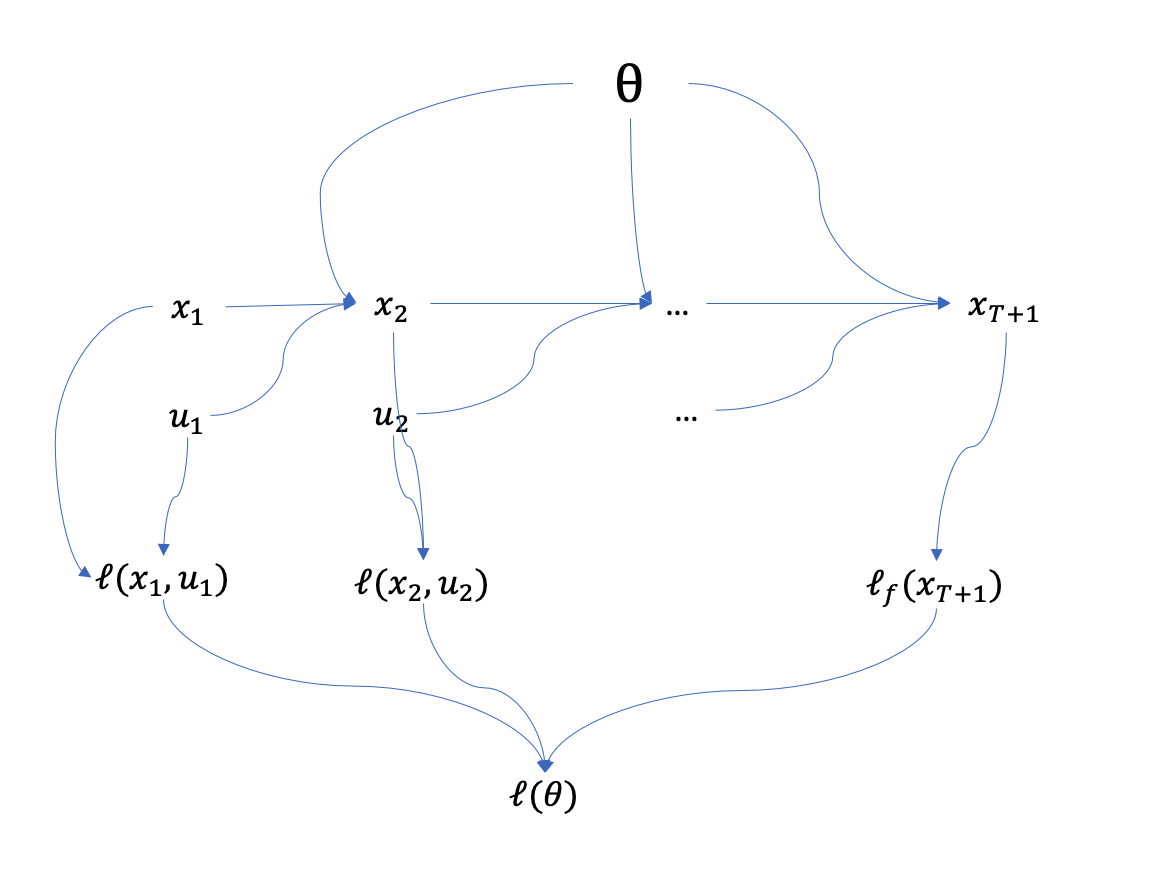
\includegraphics[width=.5\textwidth]{forward_phi.png}
\caption{Forward graph}
\label{}
\end{figure}
With all this, for any design paramter $\varphi$, we can find the optimal trajectory $(\vx_\varphi,\vu_\varphi)$. Then we proceed to update the design parameter by recording the gradients of the forward pass with the optimal trajectory $(\vx_\varphi,\vu_\varphi)$. More specifically, we have Figure \ref{fig:phi}

The experiment is on: \url{https://colab.research.google.com/drive/123VmnYlPXSXiouedK_vBS2VpI8zld_VG?usp=sharing}


\section{Discussion and future works}




\bibliographystyle{IEEEtran}
\bibliography{ref}

\end{document}
